\chapter{Déploiement et DevOps}

\section*{Introduction}
\begin{chapintro}
Ce chapitre décrit l'infrastructure de déploiement de TAC-TIC IntelliPM :
architecture cible multi-composants, conteneurisation Docker, configuration
du reverse proxy Nginx avec TLS, sécurité réseau, déploiement du microservice
IA, et pipeline CI/CD GitHub Actions. Les choix techniques visent la reproductibilité
des environnements, la séparation des préoccupations et la facilité de mise à l'échelle.
\end{chapintro}

% ============================================================
\section{Architecture de déploiement}

L'application est déployée en trois composants indépendants, chacun scalable
horizontalement de façon autonome :

\begin{table}[H]
  \centering
  \caption{Infrastructure de déploiement — Vue synthétique}
  \label{tab:infra_deploiement}
  \begin{tabularx}{\textwidth}{L{3cm}L{4cm}X}
    \toprule
    \thead{Composant} & \thead{Infrastructure} & \thead{Détails techniques} \\
    \midrule
    \rowcolor{lightgray}
    Frontend React    & Vercel (CDN mondial)    & Build Vite, déploiement automatique sur push \texttt{main} \\
    Backend Laravel   & VPS 4 vCPU / 8\,Go RAM & PHP-FPM 8.2 + Nginx, Redis, Laravel Horizon \\
    \rowcolor{lightgray}
    ML FastAPI        & VPS 2 vCPU / 4\,Go RAM & Uvicorn, modèles Joblib en mémoire \\
    Base de données   & OVH MySQL 8 managé      & Sauvegardes automatiques, réplication lecture \\
    \rowcolor{lightgray}
    WebSocket         & Laravel Reverb          & Intégré au VPS backend, port 8080 \\
    Cache             & Redis 7                 & Sessions, queues Laravel Horizon, React Query \\
    \bottomrule
  \end{tabularx}
\end{table}

\begin{figure}[H]
  \centering
  \IfFileExists{figures/ch2_architecture_distribuee.png}{%
    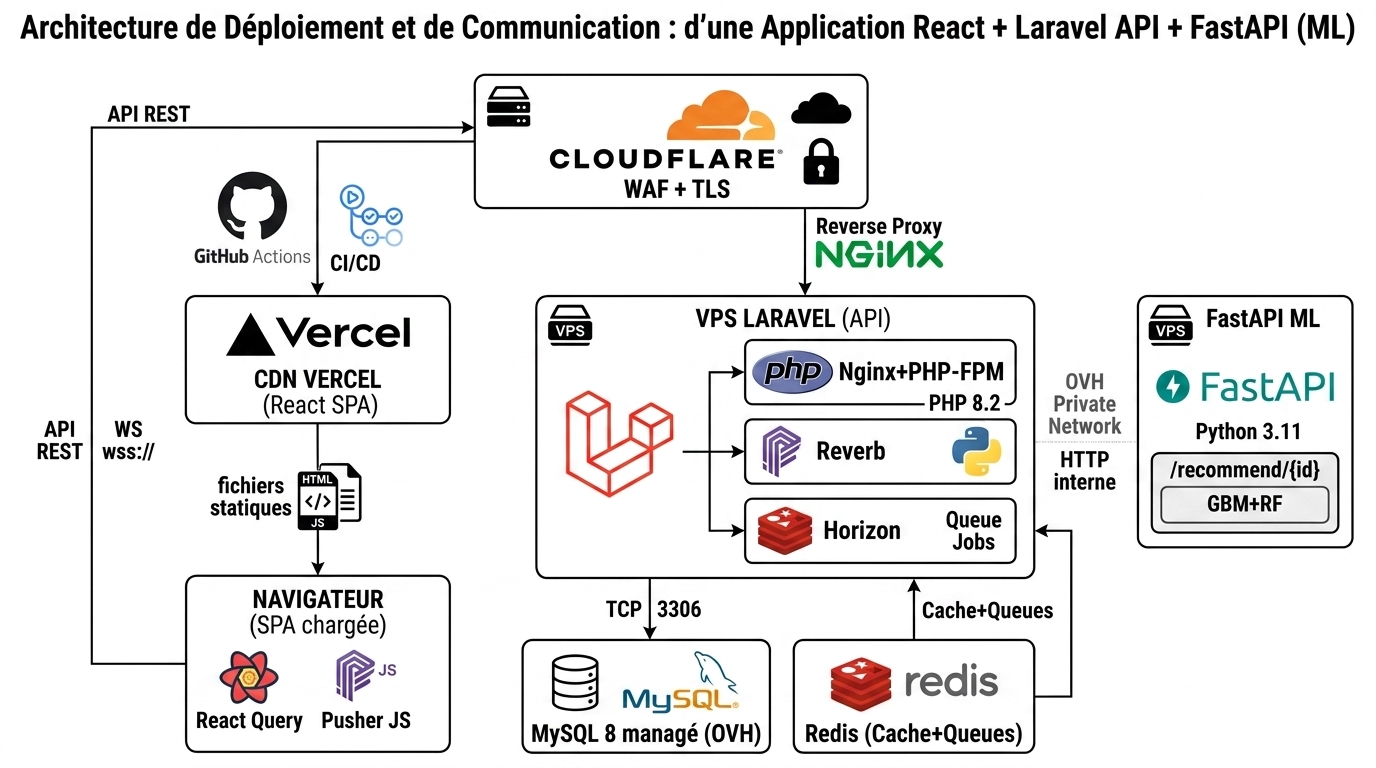
\includegraphics[width=0.92\textwidth]{figures/ch2_architecture_distribuee.png}%
  }{%
    \fbox{\parbox{0.92\textwidth}{\centering\vspace{2cm}
      \textbf{[FIGURE — Architecture de déploiement]}\\[0.4em]
      \textit{React (Vercel CDN) $\leftrightarrow$ Nginx $\leftrightarrow$ Laravel (PHP-FPM) +
      FastAPI ML $\leftrightarrow$ MySQL + Redis}
    \vspace{2cm}}}%
  }
  \caption{Architecture de déploiement — Vue globale}
  \label{fig:archi_deploiement}
\end{figure}

Cloudflare est placé en frontal devant les deux VPS : il assure le TLS (certificats
automatiques), le CDN pour les assets statiques, et la protection anti-DDoS
(rate-limiting, challenge CAPTCHA). Les requêtes API transitent par Cloudflare
Tunnel, éliminant l'exposition directe des ports serveur sur Internet.

% ============================================================
\section{Docker et Docker Compose}

La conteneurisation garantit la \textbf{parité environnements} (dev = staging = prod)
et simplifie l'intégration CI/CD. Chaque composant dispose de son propre
\texttt{Dockerfile} :

\begin{lstlisting}[style=yamlstyle,caption={Dockerfile — Backend Laravel},
  label={lst:dockerfile_laravel}]
FROM php:8.2-fpm-alpine
RUN apk add --no-cache nginx supervisor redis \
    && docker-php-ext-install pdo_mysql opcache
COPY --from=composer:2 /usr/bin/composer /usr/bin/composer
WORKDIR /var/www/html
COPY . .
RUN composer install --no-dev --optimize-autoloader \
    && php artisan config:cache \
    && php artisan route:cache \
    && php artisan view:cache
EXPOSE 9000
CMD ["php-fpm"]
\end{lstlisting}

\begin{lstlisting}[style=yamlstyle,caption={Docker Compose — Services principaux},
  label={lst:docker_compose}]
version: "3.9"
services:
  app:
    build: ./backend
    volumes: [".env:/var/www/html/.env:ro"]
    depends_on: [mysql, redis]
    networks: [tactic_net]

  nginx:
    image: nginx:1.25-alpine
    ports: ["80:80", "443:443"]
    volumes:
      - ./nginx/tactic.conf:/etc/nginx/conf.d/default.conf
      - ./ssl:/etc/nginx/ssl:ro
    depends_on: [app]
    networks: [tactic_net]

  ml:
    build: ./ml-service
    environment:
      - MODEL_PATH=/models
      - API_KEY=${ML_API_KEY}
    networks: [tactic_net]

  mysql:
    image: mysql:8.0
    environment:
      MYSQL_DATABASE: ${DB_DATABASE}
      MYSQL_ROOT_PASSWORD: ${DB_PASSWORD}
    volumes: [mysql_data:/var/lib/mysql]
    networks: [tactic_net]

  redis:
    image: redis:7-alpine
    networks: [tactic_net]

volumes:
  mysql_data:
networks:
  tactic_net:
    driver: bridge
\end{lstlisting}

% ============================================================
\section{Reverse Proxy et HTTPS}

Nginx est configuré comme reverse proxy devant PHP-FPM, gérant également la
terminaison TLS et la redirection HTTP → HTTPS :

\begin{lstlisting}[style=yamlstyle,caption={Configuration Nginx — TAC-TIC IntelliPM},
  label={lst:nginx_conf}]
server {
    listen 80;
    server_name api.tactic-intellipm.tn;
    return 301 https://$host$request_uri;
}

server {
    listen 443 ssl http2;
    server_name api.tactic-intellipm.tn;

    ssl_certificate     /etc/nginx/ssl/fullchain.pem;
    ssl_certificate_key /etc/nginx/ssl/privkey.pem;
    ssl_protocols       TLSv1.2 TLSv1.3;
    ssl_ciphers         HIGH:!aNULL:!MD5;

    root  /var/www/html/public;
    index index.php;

    location / {
        try_files $uri $uri/ /index.php?$query_string;
    }

    location ~ \.php$ {
        fastcgi_pass app:9000;
        fastcgi_param SCRIPT_FILENAME $realpath_root$fastcgi_script_name;
        include fastcgi_params;
    }

    # WebSocket Laravel Reverb
    location /app/ {
        proxy_pass http://app:8080;
        proxy_http_version 1.1;
        proxy_set_header Upgrade $http_upgrade;
        proxy_set_header Connection "upgrade";
    }
}
\end{lstlisting}

Les en-têtes de sécurité HTTP suivants sont également configurés dans Nginx :
\texttt{Strict-Transport-Security}, \texttt{X-Frame-Options: DENY},
\texttt{X-Content-Type-Options: nosniff}, \texttt{Content-Security-Policy}
et \texttt{Referrer-Policy: no-referrer}.

% ============================================================
\section{Sécurité réseau}

La stratégie de sécurité réseau repose sur plusieurs couches complémentaires :

\begin{table}[H]
  \centering
  \caption{Mesures de sécurité réseau déployées}
  \label{tab:securite_reseau}
  \begin{tabularx}{\textwidth}{L{4cm}X}
    \toprule
    \thead{Mesure} & \thead{Description et configuration} \\
    \midrule
    \rowcolor{lightgray}
    Pare-feu UFW     & Ports ouverts : 22 (SSH clé uniquement), 80, 443 ; tout le reste refusé \\
    Cloudflare WAF   & Règles OWASP Top~10, protection SQLi, XSS, traversée de répertoire \\
    \rowcolor{lightgray}
    Rate limiting    & 60 req./min par IP sur les routes d'auth ; 1\,000 req./min sur les APIs \\
    Fail2Ban         & Bannissement automatique après 5 tentatives de connexion SSH échouées \\
    \rowcolor{lightgray}
    Réseau Docker    & Tous les services sur réseau interne \texttt{tactic\_net} ; seul Nginx exposé \\
    Secrets          & Variables sensibles dans \texttt{.env} non versionné, injectées via Docker Secrets \\
    \rowcolor{lightgray}
    MySQL            & Accès restreint au réseau interne Docker ; mot de passe 32 caractères \\
    Redis            & Pas d'accès externe ; \texttt{requirepass} configuré \\
    \bottomrule
  \end{tabularx}
\end{table}

% ============================================================
\section{Déploiement du microservice IA}

Le microservice FastAPI est déployé dans son propre conteneur avec une configuration
adaptée aux contraintes de performance :

\begin{lstlisting}[style=yamlstyle,caption={Dockerfile — Microservice ML FastAPI},
  label={lst:dockerfile_ml}]
FROM python:3.11-slim
WORKDIR /app
COPY requirements.txt .
RUN pip install --no-cache-dir -r requirements.txt
COPY app/ ./app/
COPY models/ ./models/
# Pre-load models at build time
RUN python -c "import joblib; joblib.load('models/voting_clf.joblib')"
EXPOSE 8000
CMD ["uvicorn", "app.main:app", "--host", "0.0.0.0",
     "--port", "8000", "--workers", "2"]
\end{lstlisting}

Les modèles Joblib sont chargés en mémoire une seule fois au démarrage
(\textit{startup event} FastAPI), réduisant la latence d'inférence à
moins de \textbf{45\,ms} en médiane. La clé API partagée avec Laravel est
validée via un middleware FastAPI sur chaque requête :

\begin{lstlisting}[style=pythonstyle,caption={Middleware d'authentification FastAPI},
  label={lst:ml_auth_middleware}]
from fastapi import Request, HTTPException
import os

async def api_key_middleware(request: Request, call_next):
    key = request.headers.get("X-ML-API-Key")
    if key != os.environ["ML_API_KEY"]:
        raise HTTPException(status_code=401, detail="Unauthorized")
    return await call_next(request)
\end{lstlisting}

% ============================================================
\section{Pipeline CI/CD — GitHub Actions}

Le pipeline d'intégration et déploiement continus orchestre cinq étapes séquentielles :

\begin{lstlisting}[style=yamlstyle,caption={Pipeline GitHub Actions — .github/workflows/deploy.yml},
  label={lst:github_actions}]
name: CI/CD — TAC-TIC IntelliPM
on:
  push:
    branches: [main]

jobs:
  test-backend:
    runs-on: ubuntu-latest
    steps:
      - uses: actions/checkout@v4
      - uses: shivammathur/setup-php@v2
        with: { php-version: '8.2' }
      - run: composer install && php artisan test

  sonarcloud:
    needs: test-backend
    runs-on: ubuntu-latest
    steps:
      - uses: actions/checkout@v4
      - uses: SonarSource/sonarcloud-github-action@master
        env:
          GITHUB_TOKEN: ${{ secrets.GITHUB_TOKEN }}
          SONAR_TOKEN: ${{ secrets.SONAR_TOKEN }}

  build-deploy:
    needs: sonarcloud
    runs-on: ubuntu-latest
    steps:
      - uses: actions/checkout@v4
      - run: docker build -t tactic/backend ./backend
      - run: docker build -t tactic/ml-service ./ml-service
      - name: Deploy to VPS
        uses: appleboy/ssh-action@v1
        with:
          host: ${{ secrets.VPS_HOST }}
          key:  ${{ secrets.VPS_SSH_KEY }}
          script: |
            cd /opt/tactic
            git pull origin main
            docker compose pull
            docker compose up -d --build
            docker compose exec app php artisan migrate --force
\end{lstlisting}

\begin{chapconclusion}
La chaîne CI/CD complète (lint → tests → SonarCloud → build Docker → déploiement
SSH automatique) garantit qu'aucune régression ne peut atteindre l'environnement
de production. L'architecture Docker Compose assure la parité des environnements,
tandis que Cloudflare, Nginx et UFW forment une protection multicouche. Le chapitre
suivant présente les stratégies de tests adoptées pour valider la qualité du code
à tous les niveaux.
\end{chapconclusion}
